%\documentclass[envcountsect,11pt,trans]{beamer}
\documentclass[11pt,aspectratio=169]{beamer}
\usepackage[english]{babel}
\usepackage[ansinew]{inputenc}
\usepackage{times}
\usepackage{xcolor}
\usepackage{graphicx}
\usepackage{rotating}
\usepackage{bbding,pifont} % two dingbat fonts
\usepackage{amsmath}
\usepackage{amsfonts}
\usepackage{amssymb}
\usepackage{fancybox}
\usepackage{epstopdf}
\usepackage{eso-pic}
%\usepackage[round]{natbib}
\usepackage{ngerman}
\usepackage{tcolorbox}
\usepackage{colortbl}
%\usepackage[authordate,bibencoding=auto,strict,backend=biber]{biblatex-chicago}
%\usepackage{natbib}
%\usepackage[style=bath, backend=biber]{biblatex}
\usepackage{ulem}
\usepackage{tikz}
\usepackage{booktabs}
\usepackage{longtable}
\usepackage{hyperref}
\usepackage{array}
\usepackage{appendixnumberbeamer}
\usepackage[T1]{fontenc}
\usepackage{adjustbox}
\usepackage{listings}
\usepackage{uarial}
\usepackage{fancyvrb}
\usepackage{subfigure}
\renewcommand{\familydefault}{\sfdefault}

\newcommand*\circled[1]{\tikz[baseline=(char.base)]{
            \node[shape=circle,draw,inner sep=2pt] (char) {#1};}}
\newcommand{\E}{\operatorname{E}}
\newcommand{\Var}{\operatorname{Var}}
\newcommand{\overbar}[1]{\mkern 1.5mu\overline{\mkern-1.5mu#1\mkern-1.5mu}\mkern 1.5mu}
\DeclareMathOperator*{\argmin}{arg\,min}
\DeclareMathOperator*{\argmax}{arg\,max}
% \use\smallpackage{pgfpages}
% \pgfpagesuselayout{4 on 1}[a4paper,border shrink=10mm,landscape]

%\xdefinecolor{MyColor}{rgb}{0.14,0.17,0.52}
%\xdefinecolor{MyColor}{rgb}{0.29,0.53,0.82}
%\xdefinecolor{MyBlue}{rgb}{0.14,0.17,0.52}
%\xdefinecolor{MyGreen}{rgb}{0.70,0.78,0.14}
%\xdefinecolor{MyAlert}{rgb}{0.29,0.53,0.82}
%\colorlet{mystructure}{MyColor}
%\usecolortheme[named=mystructure]{structure}
%\setbeamercolor{alerted text}{fg=MyAlert}
\definecolor{Black}{RGB}{0,0,0}
\definecolor{RedGIZ}{RGB}{200,15,15}
\setbeamercolor{title}{fg=black}
\setbeamercolor{section in toc}{fg=black}
\setbeamercolor{subsection in toc}{fg=black}
\setbeamercolor{frametitle}{fg=Black}
\setbeamercolor{tableofcontents}{fg=Black}

%\usetheme{Boadilla}
%\usetheme{Madrid}
%\useoutertheme{infolines}
%\usecolortheme{whale}
%\usecolortheme{lily}
\renewcommand{\inserttitlegraphic}{
\parbox[b][2.5cm][t]{4cm}{
\includegraphics[width = 4cm, keepaspectratio]{pictures/GIZ_Logo.png}}  \hspace{0.1cm} \parbox[b][2.5cm][t]{4cm}{
\includegraphics[width = 4cm, keepaspectratio]{pictures/IWH_Logo_RGB_DE_Grossformat.png}} \hfill \parbox[b][2.5cm][t]{3.21cm}{
\includegraphics[keepaspectratio,width=4.00cm]{pictures/seperationbar.png} \\ \includegraphics[width = 4cm, keepaspectratio]{pictures/BMWI_logo.png}}
}
\defbeamertemplate*{title page}{customized}[1][]
{	
	\vspace{2.75cm}
  \usebeamerfont{title}\begin{center}\textbf{\inserttitle}\end{center}\par
  \usebeamerfont{subtitle}\begin{center}\usebeamercolor[fg]{subtitle}\insertsubtitle\end{center}\par
  \usebeamerfont{author}\insertauthor $\, \vert$ \usebeamerfont{date}\insertdate \par
  \usebeamerfont{institute}\insertinstitute\par
	\vspace{0.25cm}
  \usebeamercolor[fg]{titlegraphic}\inserttitlegraphic


}
\setbeamerfont{subtitle}{size=\normalsize}
\setbeamerfont{author}{size=\tiny}
\setbeamerfont{date}{size=\tiny}
\setbeamerfont{institute}{size=\tiny}

\setbeamercovered{transparent}

\setbeamertemplate{footline}[text line]{%
  \parbox{\linewidth}{\vspace*{-8pt} $\vert$ \hspace{1mm} \today \hspace{1mm} $\vert$ \hfill}}
\setbeamertemplate{navigation symbols}{}

\linespread{1.2}





\mode<presentation>{
    \setbeamertemplate{itemize item}{\color{RedGIZ}$\blacksquare$}
    \setbeamertemplate{itemize subitem}{\color{RedGIZ}$\blacktriangleright$}
		}
\title[DGE-CRED]{Dynamic General Equilibrium Model for Climate Resilient Economic Development}
%\subtitle[]{Training}

\author[Christoph Schult]{Andrej Drygalla and Christoph Schult} \date[June 2020]{June 2020}

\institute[IWH]{Halle Institute for Economic Research}

 
\logo{\begin{tabular}{c}
\includegraphics[keepaspectratio,width=1.00cm]{pictures/seperationbar.png} \\ 
\includegraphics[keepaspectratio,width=1.00cm]{pictures/GIZ_Logo}\end{tabular}}

\usepackage[style=authoryear-comp,maxbibnames=9,maxcitenames=2,backend=bibtex]{biblatex}
\bibliography{references}

\begin{document}
%\footnotesize
\usebackgroundtemplate{
\vbox to \paperheight{\vspace{0.1cm}\hbox to \paperwidth{\hfil
\includegraphics[width=0.975\paperwidth,height = 0.7\paperheight]{pictures/BackgroundGIZ.jpg}\hfil}\vfil
}}
\begin{frame}<presentation>[noframenumbering,plain]
  \titlepage
\end{frame}
\usebackgroundtemplate{
}
\begin{frame}<presentation>[noframenumbering]
  \tableofcontents[sectionstyle=show/show, subsectionstyle=show/show/hide]
\end{frame}

\section{Introduction to Dynare}
\subsection{What is Dynare?}
\begin{frame}<presentation>
\frametitle{What is Dynare?}
  \begin{itemize}
		\item dynare is an open-source program for dynamic general equilibrium modeling
		\item mainly a collection of different functions written for Matlab
		\item preprocessor translates mod files into matlab code.
	\end{itemize}
\end{frame}


\subsection{The structure of a Mod File}
\begin{frame}<presentation>
\frametitle{Structure of a Mod File}
  \begin{itemize}
		\item var block declares endogenous variables 
		\item params block
	\end{itemize}
\end{frame}

\begin{frame}<presentation>[fragile]
\frametitle{Declaration of endogenous variables}
  \begin{lstlisting}
		var 
		k $k$ (long_name = 'capital'),
		c $c$ (long_name = 'consumption'),
		h $h$ (long_name = 'hours worked'),
		epsil $\epsilon$ (long_name = 'tfp shock')
		;
	\end{lstlisting}
\end{frame}

\begin{frame}<presentation>[fragile]
\frametitle{Declaration of endogenous variables}
  \begin{verbatim}
		var 
		k $k$ (long_name = 'capital'),
		c $c$ (long_name = 'consumption'),
		h $h$ (long_name = 'hours worked'),
		epsil $\epsilon$ (long_name = 'tfp shock')
		;
	\end{verbatim}
\end{frame}



\subsection{Implementation of a Neoclassical Growth Model}

\section{DGE-CRED Model}

\subsection{Introduction}
\begin{frame}[plain]
\frametitle{Introduction}
\begin{itemize}
\item A dynamic general equilibrium model with optimizing agents
\item We differentiate between regions and economic activities.
\item Our model is implemented in the open source environment \href{https://www.dynare.org/}{Dynare} and can be run using Matlab or Octave.
\begin{itemize}
	\item Sectors in the model correspond to economic activities and the classification by the General Statistical Office (GSO).
	\item Regions are based on the statistical regions.
\end{itemize}
\item We extend the approach by \cite{nordhaus1993optimal} to model the impact of climate change through damage functions.
\end{itemize}
\end{frame}

\begin{frame}[plain]
\frametitle{Model Structure}
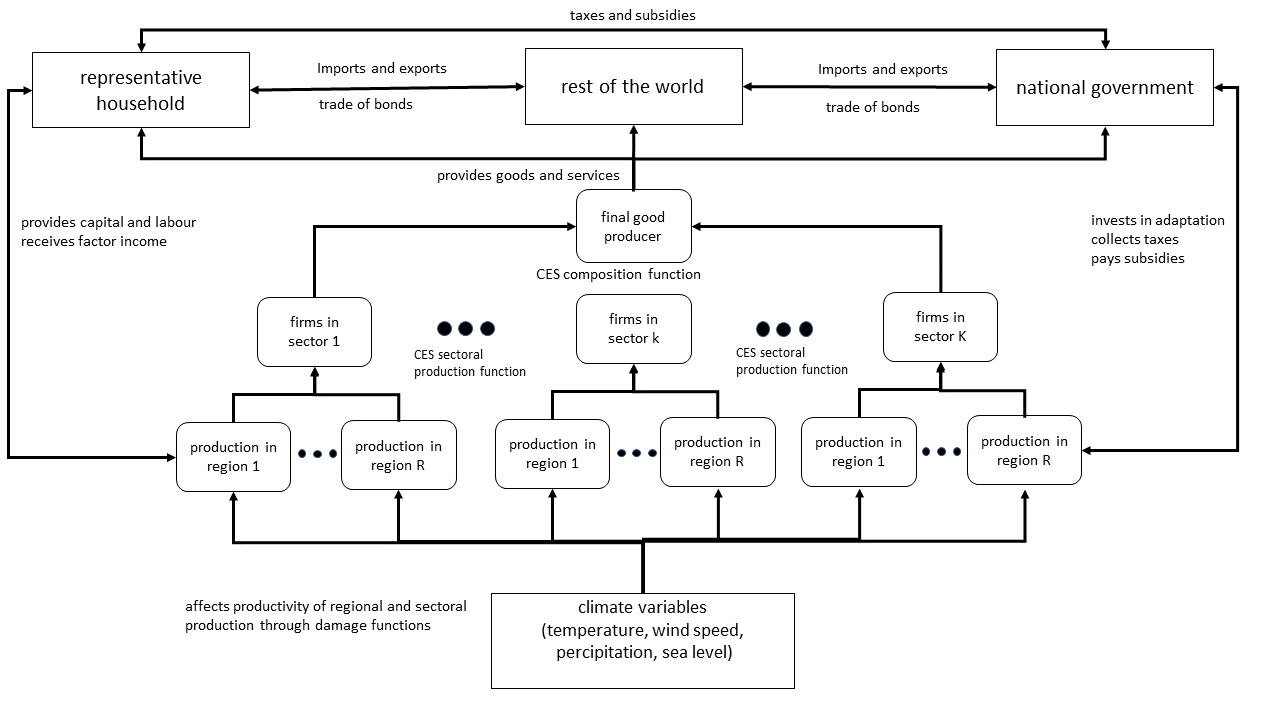
\includegraphics[width = 1\textwidth]{pictures/Model_Structure.png}
\end{frame}


\subsection{Demand}
\begin{frame}
\frametitle{Households}
\scriptsize
\begin{itemize}
\item representative households $h$ providing labour $N$ and capital $K$ to domestic firms $f$
\item maximize discounted utility over an infinite horizon by choosing consumption $C_t(h)$, capital $K_{k,r,t+1}(h)$, investments $I_{k,r,t}(h)$, labour $N_{k,r,t}(h)$ and foreign net wealth $B_{t+1}$
\item the optimization problem of the representative household is
\begin{align*}
 & \underset{C_t(h), \, K_{k,r,t+1}(h), \, I_{k,r,t}(h), , \, N_{k,r,t}(h), \, B_{t+1}}{\mbox{max}} \sum_{t=0}^{\infty} \beta^{t} \left(\frac{C_{t}(h)^{1 - \sigma^{C}}}{1 - \sigma^{C}} - \sum_{k=1}^{K} \sum_{r=1}^{R} A^{N}_{k,r,t} \, \phi^{L}_{k,r} \frac{N_{k,r,t}(h)^{1+\sigma^{L}}}{1+\sigma^{L}} \right) \\
\mbox{s.t.} & P_{t} \, C_{t}(h) \, (1 + \tau^{C}) + \sum_{k=1}^{K} \sum_{r=1}^{R} P_{k,r,t} I_{k,r,t}(h) + B_{t+1}(h) = \\
 & \sum_{k=1}^{K} \sum_{r=1}^{R} (1 - \tau^{N}) \, W_{k,r,t} N_{k,r,t}(h) + \sum_{k=1}^{K} \sum_{r=1}^{R} P_{k,r,t} \, r_{k,r,t} \, (1 - \tau^{K}) \, K_{k,r,t}(h) + S^{f}_{t} \, \phi^{B}_{t} \, (1 + r^{f}_{t} )\, B_{t}(h)
 %K_{k,r,t+1} = (1 - \delta - D^K_{k,r,t}) \, K_{k,r,t} - I_{k,r,t} \, \Gamma\left(\frac{I_{k,r,t}}{I_{k,r,t-1}}\right).
\end{align*}
\end{itemize}
\end{frame}


\begin{frame}
\frametitle{Households Lagrangian}
\scriptsize
\begin{itemize}
\item We set-up the Lagrangian for the optimization problem to derive the first order conditions.
\begin{align*}
& \sum_{t=0}^{\infty} \beta^{t} \Bigg[ \left(\frac{C_{t}(h)^{1 - \sigma^{C}}}{1 - \sigma^{C}} - \sum_{k=1}^{K} \sum_{r=1}^{R} A^{N}_{k,r,t} \, \phi^{L}_{k,r} \frac{N_{k,r,t}(h)^{1+\sigma^{L}}}{1+\sigma^{L}} \right) \\
& - \lambda_{t}(h) \Big(P_{t} \, C_{t}(h) \, (1 + \tau^{C}) + \sum_{k=1}^{K} \sum_{r=1}^{R} P_{k,r,t} I_{k,r,t}(h) + B_{t+1}(h) - \sum_{k=1}^{K} \sum_{r=1}^{R} (1 - \tau^{N}) \, W_{k,r,t} N_{k,r,t}(h) \\
& - \sum_{k=1}^{K} \sum_{r=1}^{R} P_{k,r,t} \, r_{k,r,t} \, (1 - \tau^{K}) \, K_{k,r,t}(h) - S^{f}_{t} \, \phi^{B}_{t} \, (1 + r^{f}_{t} )\, B_{t}(h) \Big) \\
& - \sum_{k=1}^{K} \sum_{r=1}^{R} \lambda_{t}(h) \omega^{I}_{k,r,t}(h) \left\lbrace K_{k,r,t+1} - (1 - \delta - D^K_{k,r,t}) \, K_{k,r,t} - I_{k,r,t} \, \Gamma\left(\frac{I_{k,r,t}}{I_{k,r,t-1}}\right) \right\rbrace\Bigg] .
\end{align*}
\end{itemize}
\end{frame}


\begin{frame}
\frametitle{Households First Order Conditions - Intratemporal}
\scriptsize
\begin{itemize}
\item Marginal utility of consumption
\begin{align*}
\lambda_{t} =\frac{C_{t}(h)^{-\sigma^{C}}}{P_{t}\, (1 + \tau^C)}
\end{align*}
\item Labour supply curve
\begin{align*}
\phi^{L}_{k,r} \, A^{N}_{k,r,t} \, N_{k,r,t}(h)^{\sigma^{L}} = \lambda_{t}(h) \, W_{k,r,t} \, (1 - \tau^{N}) \\
\end{align*}
\end{itemize}
\end{frame}


\begin{frame}
\frametitle{Households First Order Conditions - Intertemporal}
\scriptsize
\begin{itemize}
\item Euler equation for foreign bonds
\begin{align*}
\lambda_{t+1} \, \beta \, S^{f}_{t+1} \, \phi^{B}_{t+1} \left(1+{{r^{f}}_{t+1}}\right) = \lambda_{t} \\
\end{align*}
\item Euler equation for capital
\begin{align*}
\lambda_{t+1}(h) \, \beta \, \left(P_{k,r,t+1} \, r_{k,r,t+1} \, (1 - \tau^K) + (1 - \delta - D^{K}_{k,r,t+1}) \, \omega^{I}_{k,r,t+1} \right) = \lambda_{t}(h) \, \omega^{I}_{k,r,t}.
\end{align*}
\item Euler equation for investment
\begin{align*}
P_{k,r,t} \, \lambda_{t}(h) = \lambda_{t}(h) \, \omega^{I}_{k,r,t} \, \left(\Gamma(\frac{I_{k,r,t}}{I_{k,r,t-1}}) + \frac{\partial \Gamma(\frac{I_{k,r,t}}{I_{k,r,t-1}})}{\partial (\frac{I_{k,r,t}}{I_{k,r,t-1}})} \, \frac{I_{k,r,t}}{I_{k,r,t-1}} \right) - \beta \lambda_{t+1}(h) \, \omega^{I}_{k,r,t+1} \, \frac{\partial \Gamma(\frac{I_{k,r,t+1}}{I_{k,r,t}})}{\partial (\frac{I_{k,r,t+1}}{I_{k,r,t}})} \, \left(\frac{I_{k,r,t+1}}{I_{k,r,t}}\right)^2
\end{align*}
\item Investment adjustment cost
\begin{align*}
\Gamma(\frac{I_{k,r,t}}{I_{k,r,t-1}}) = 3 - exp\left\lbrace\sqrt{\phi^{K}/2}\left(\frac{I_{k,r,t}}{I_{k,r,t-1}}-1\right\rbrace\right) - exp\left\lbrace-\sqrt{\phi^{K}/2}\left(\frac{I_{k,r,t}}{I_{k,r,t-1}}-1\right)\right\rbrace
\end{align*}
\end{itemize}
\end{frame}

\begin{frame}
\frametitle{Households First Order Conditions - Intertemporal}
\scriptsize
\begin{itemize}
\item Euler equation for capital
\begin{align*}
\lambda_{t+1}(h) \, \beta \, \left(P_{k,r,t+1} \, r_{k,r,t+1} \, (1 - \tau^K) + (1 - \delta - D^{K}_{k,r,t+1}) \, \omega^{I}_{k,r,t+1} \right) = \lambda_{t}(h) \, \omega^{I}_{k,r,t}.
\end{align*}
\item Euler equation for investment
\begin{align*}
P_{k,r,t} \, \lambda_{t}(h) = \lambda_{t}(h) \, \omega^{I}_{k,r,t} \, \left(\Gamma(\frac{I_{k,r,t}}{I_{k,r,t-1}}) + \frac{\partial \Gamma(\frac{I_{k,r,t}}{I_{k,r,t-1}})}{\partial (\frac{I_{k,r,t}}{I_{k,r,t-1}})} \, \frac{I_{k,r,t}}{I_{k,r,t-1}} \right) - \beta \lambda_{t+1}(h) \, \omega^{I}_{k,r,t+1} \, \frac{\partial \Gamma(\frac{I_{k,r,t+1}}{I_{k,r,t}})}{\partial (\frac{I_{k,r,t+1}}{I_{k,r,t}})} \, \left(\frac{I_{k,r,t+1}}{I_{k,r,t}}\right)^2
\end{align*}
\end{itemize}
\end{frame}


\begin{frame}
\frametitle{Rest of the world}
\scriptsize
\begin{itemize}
\item Euler equation foreign bonds
\begin{align*}
\lambda_{t+1} \, \beta \, S^{f}_{t+1} \, \phi^{B}_{t+1} \left(1+{{r^{f}}_{t+1}}\right) = \lambda_{t}
\end{align*}
\item Effective exchange rate $S^f$ and the world interest rate $r^f$.
\item The required interest rate is above the world interest rate if the foreign debt ($B_{t+1}<0$)/ foreign claims ($B_{t+1}>0$) relative to GDP increases/decreases and future net exports relative to GDP will decrease. 
\begin{align*}
\phi^{B}_{t+1} = exp \left(-\phi^B \,(S^{f}_{t+1} \, r^{f}_{t+1} \, \frac{B_{t+1}}{Y_{t+1}}+\frac{NX_{t+1}}{Y_{t+1}})\right)
\end{align*}
\end{itemize}
\end{frame}


\begin{frame}
\frametitle{Government Budget Constraint}
\scriptsize
\begin{itemize}
\item We are interested in different policy measures taken by the government to adapt to a new climate regime. 
\item Government behaviour is not a result of an optimization problem. 
\begin{align*}
G_{t} + \sum_{k}^{K} \sum_{r}^{R} G^{A}_{k,r,t} + B^G_{t+1} =& \sum_{k}^{K} \sum_{r}^{R} \, \left\lbrace (\tau^{K} + \tau_{r,k,t}^{K}) \, P_{k,r,t} \, r_{k,r,t} \, K_{k,r,t} + (\tau^{N} + \tau_{k,r,t}^{N}) \, W_{k,r,t} \, N_{k,r,t} \, Pop_{t} \right\rbrace \nonumber \\
& + (1 + r^{f}_{t}) \, S^{f}_{t} \phi^{B}_{t} \, B^G_{t}
\end{align*}
\end{itemize}
\end{frame}

\begin{frame}
\frametitle{Government Policy Instruments}
\scriptsize
\begin{itemize}
\item Governments can invest into adaptation capital stocks
\begin{align*}
K^{A,z}_{k,r,t+1} = \eta^{A,z}_{k,r,t}
\end{align*}
\item Evolution of adaptation capital stocks
\begin{align*}
K^{A,z}_{k,r,t+1} = (1 - \delta_{K^{A,z},k,r}) \, K^{A,z}_{k,r,t} + G^{A,z}_{k,r,t} \nonumber \\
\end{align*}
\item Tax on capital expenditures paid by firms
\begin{align*}
\tau^{K}_{k,r,t} = \tau^{K}_{k,r,0} + \eta^{\tau^{K}}_{k,r,t} \nonumber \\
\end{align*}
\item Tax rate on wage bill paid by firms
\begin{align*}
\tau^{N}_{k,r,t} = \tau^{N}_{k,r,0} + \eta^{\tau^{N}}_{k,r,t} \nonumber \\
\end{align*}
\end{itemize}
\end{frame}

\begin{frame}
\frametitle{Resource constraint}
\scriptsize
\begin{itemize}
\item Households and government use domestic final goods $Y_t$ produced by firms for consumption, investment and for exports $X_{t}$ and can also use imports $M_t$ for consumption and investment
\begin{align}
Y_{t} = C_{t} + I_{t} + G_{t} + \underbrace{X_{t} - M_{t}}_{NX_{t}}
\end{align}
\item The aggregation of the budget constraints of the representative households also states that positive net exports are used to increase net financial wealth to the rest of the world.
\begin{align}
NX_t = B_{t+1} - (1 + r^{f}_{t}) S^{f}_{t} \phi^B_{t} B_{t}
\end{align}
\end{itemize}
\end{frame}

%
%
\subsection{Production}

\begin{frame}
\frametitle{Sectoral Decomposition}
\scriptsize
\begin{itemize}
\item Final domestic goods $Y_{t}$ are created combining goods from different sectors $Y_{k,t}$ using a CES production function.
\begin{align}
\underset{Y_{k,t}}{\mathrm{min}} & \sum_{k} Y_{k,t} \, P_{k,t} \\ 
Y_{t} &= \left(\sum_{k} {\omega^{Q}_{k}}^{\frac{1}{\eta^Q}} Y_{k,t}^{\frac{\eta^Q-1}{\eta^Q}} \right)^{\frac{\eta^Q}{\eta^Q-1}}
\end{align}

\item Therefore, the demand for sectoral products correspond to the first order conditions of the above optimization problem. 
\begin{align*}
\frac{P_{k,t}}{P_{t}} &= {\omega^{Q}_{k}}^{\frac{1}{\eta^Q}} \left(\frac{Y_{k,t}}{Y_{t}}\right)^{\frac{-1}{\eta^Q}}
\end{align*}
\end{itemize}
\end{frame}



\begin{frame}
\frametitle{Regional Decomposition}
\scriptsize
\begin{itemize}
\item In order to model regional economic activity we further decompose the production process on a regional level.
\begin{align*}
\underset{Y_{k,r,t}}{\mathrm{min}} & \sum_{k} Y_{k,r,t} \, P_{k,r,t} \\ 
Y_{k,t} &= \left(\sum_{k} {\omega^{Q}_{k,r}}^{\frac{1}{\eta^Q_{k}}} Y_{k,r,t}^{\frac{\eta^Q_{k}-1}{\eta^Q_{k}}} \right)^{\frac{\eta^Q_{k}}{\eta^Q_{k}-1}}
\end{align*}
\item Demand for sectoral and regional products correspond to the first order conditions of the above optimization problem.
\begin{align*}
\frac{P_{k,r,t}}{P_{k,t}} &= {\omega^{Q}_{k,r}}^{\frac{1}{\eta^{Q}_{k}}} \left(\frac{Y_{k,r,t}}{Y_{k,t}}\right)^{\frac{-1}{\eta^{Q}_{k}}}
\end{align*}
\end{itemize}
\end{frame}

\begin{frame}
\frametitle{Regional Production}
\scriptsize
\begin{itemize}
\item At the regional and sectoral level are representative firms maximizing profits using capital $K_{k,r,t}$ and labour $L_{k,r,t} = N_{k,r,t} \, Pop_{t}$ provided by households to produce products. 
\item They charge a price $P_{k,r,t}$ for their products and have to pay households wages $W_{k,r,t}$, interest on rented capital $P_{r,k,t} \, r_{r,k,t}$, taxes related to the wage bill $\tau^{N}_{r,k,t}$ and on capital expenditure $\tau^{K}_{r,k,t}$.
\item Representative firms have access to a regional and sector specific constant elasticity of substitution production function.
\item The productivity of capital and labour of a firm in one sector and region depends on the climate variables, and the adaption measures by the government represented by a damage function affecting total factor productivity $A_{k,r,t}$ by $D_{k,r,t} = D_{k,r}\left(T_{r,t}, \, PREC_{r,t}, \, WS_{r,t}, \, SL_{r,t}, \, CYC_{r,t}, \, DRO_{r,t}, \, G^{A}_{r,k,t} \right)$.
\item Further, we explicitly differentiate between climate induced damages affecting labour productivity $D_{N,k,r,t}$ and capital depreciation $D_{K,k,r,t}$. 
\item As in \cite{nordhaus1993optimal}, we assume a polynomial functional form of the damage functions, but the damages are different across regions and sectors.
\end{itemize}
\end{frame}


\begin{frame}
\frametitle{Damages on TFP}
\tiny
\begin{align*}
{{D_{k,r}}_{t}} &= \Big\lbrace \nonumber \\
 & (\underbrace{{{a_{T,1,k,r}}} \, {{T_{r}}_{t}}+{{a_{T,2,k,r}}}\, \left({T_{r}}_{t}\right)^{a_{T,3,k,r}}}_{\mbox{impact of temperature}})  \, \underbrace{exp(-\phi^{G^{A,T}}_{k,r} K^{A,T}_{k,r,t})}_{\mbox{impact of adaptation}} \, 
 + (\underbrace{{{a_{SL,1,k,r}}}\, {{SL}_{t}}+{{a_{SL,2,k,r}}}\, \left({SL}_{t}\right)^{{{a_{SL,3,k,r}}}}}_{\mbox{impact of sea level}})   \, \underbrace{I(SL > \frac{K^{A,SL}_{k,r,t}}{\phi^{G^{A,SL}}_{k,r}})}_{\mbox{impact of adaptation}} \\
& +  (\underbrace{{{a_{WS,1,k,r}}}\, {{WS_{r}}_{t}}+{{a_{WS,2,k,r}}}\, \left({WS_{r}}_{t}\right)^{{{a_{WS,3,k,r}}}}}_{\mbox{impact of wind speed}}) \, \underbrace{exp(-\phi^{G^{A,WS}}_{k,r} K^{A,WS}_{k,r,t})}_{\mbox{impact of adaptation}} \\
& + (\underbrace{{{a_{PREC,1,k,r}}} \, {{PREC_{r}}_{t}}+{{a_{PREC,2,k,r}}}\, \left({PREC_{r}}_{t}\right)^{{{a_{PREC,3,k,r}}}}}_{\mbox{impact of precipitation}}) \, \underbrace{exp(-\phi^{G^{A,PREC}}_{k,r} K^{A,PREC}_{k,r,t})}_{\mbox{impact of adaptation}} \nonumber \\
& +  (\underbrace{{{a_{CYC,1,k,r}}}\, {{CYC_{r}}_{t}}+{{a_{CYC,2,k,r}}}\, \left({CYC_{r}}_{t}\right)^{{{a_{CYC,3,k,r}}}}}_{\mbox{impact of cyclones}}) \, \underbrace{exp(-\phi^{G^{A,CYC}}_{k,r} K^{A,CYC}_{k,r,t})}_{\mbox{impact of adaptation}} \\
& +  (\underbrace{{{a_{DRO,1,k,r}}} \, {{DRO_{r}}_{t}}+{{a_{DRO,2,k,r}}}\, \left({DRO_{r}}_{t}\right)^{{{a_{DRO,3,k,r}}}}}_{\mbox{impact of droughts}}) \, \underbrace{exp(-\phi^{G^{A,DRO}}_{k,r} K^{A,DRO}_{k,r,t})}_{\mbox{impact of adaptation}} \\
& \Big\rbrace.
\end{align*}
\end{frame}

\begin{frame}
\frametitle{Damages on Labour Productivity}
\tiny
\begin{align*}

%{{D^{N}_{k,r}}_{t}}=& \Big( \nonumber \\
%&\underbrace{{{a^{N}_{T,1,k,r}}} \, {{T_{r}}_{t}}+{{a^{N}_{T,2,k,r}}}\, \left({T_{r}}_{t}\right)^{a^{N}_{T,3,k,r}}}_{\mbox{impact of temperature}} + 
%\underbrace{{{a^{N}_{SL,1,k,r}}}\, {{SL}_{t}}+{{a^{N}_{SL,2,k,r}}}\, \left({SL}_{t}\right)^{{{a^{N}_{SL,3,k,r}}}}}_{\mbox{impact of sea level}} \nonumber \\
%+ & \underbrace{{{a^{N}_{WS,1,k,r}}}\, {{WS_{r}}_{t}}+{{a^{N}_{WS,2,k,r}}}\, \left({WS_{r}}_{t}\right)^{{{a^{N}_{WS,3,k,r}}}}}_{\mbox{impact of wind speed}} 
%+ (\underbrace{{{a^{N}_{PREC,1,k,r}}} \, {{PREC_{r}}_{t}}+{{a^{N}_{PREC,2,k,r}}}\, \left({PREC_{r}}_{t}\right)^{{{a^{N}_{PREC,3,k,r}}}}}_{\mbox{impact of precipitation}}) \,  \nonumber \\
%+ & \underbrace{{{a^{N}_{CYC,1,k,r}}}\, {{CYC_{r}}_{t}}+{{a^{N}_{CYC,2,k,r}}}\, \left({CYC_{r}}_{t}\right)^{{{a^{N}_{CYC,3,k,r}}}}}_{\mbox{impact of cyclones}}
%+ \underbrace{{{a^{N}_{DRO,1,k,r}}} \, {{DRO_{r}}_{t}}+{{a^{N}_{DRO,2,k,r}}}\, \left({DRO_{r}}_{t}\right)^{{{a^{N}_{DRO,3,k,r}}}}}_{\mbox{impact of droughts}} \nonumber \\
%&\Big). \\
%{{D^{K}_{k,r}}_{t}}=& \Big( \nonumber \\
%&\underbrace{{{a^{K}_{T,1,k,r}}} \, {{T_{r}}_{t}}+{{a^{K}_{T,2,k,r}}}\, \left({T_{r}}_{t}\right)^{a^{K}_{T,3,k,r}}}_{\mbox{impact of temperature}}+ \underbrace{{{a^{K}_{SL,1,k,r}}}\, {{SL}_{t}}+{{a^{K}_{SL,2,k,r}}}\, \left({SL}_{t}\right)^{{{a^{K}_{SL,3,k,r}}}}}_{\mbox{impact of sea level}} \nonumber \\
%+ & \underbrace{{{a^{K}_{WS,1,k,r}}}\, {{WS_{r}}_{t}}+{{a^{K}_{WS,2,k,r}}}\, \left({WS_{r}}_{t}\right)^{{{a^{K}_{WS,3,k,r}}}}}_{\mbox{impact of wind speed}}
%+ \underbrace{{{a^{K}_{PREC,1,k,r}}} \, {{PREC_{r}}_{t}}+{{a^{K}_{PREC,2,k,r}}}\, \left({PREC_{r}}_{t}\right)^{{{a^{K}_{PREC,3,k,r}}}}}_{\mbox{impact of precipitation}} \nonumber \\
%+ & \underbrace{{{a^{K}_{CYC,1,k,r}}}\, {{CYC_{r}}_{t}}+{{a^{K}_{CYC,2,k,r}}}\, \left({CYC_{r}}_{t}\right)^{{{a^{K}_{CYC,3,k,r}}}}}_{\mbox{impact of cyclones}}
%+ \underbrace{{{a^{K}_{DRO,1,k,r}}} \, {{DRO_{r}}_{t}}+{{a^{K}_{DRO,2,k,r}}}\, \left({DRO_{r}}_{t}\right)^{{{a^{K}_{DRO,3,k,r}}}}}_{\mbox{impact of droughts}} \nonumber \\
%&\Big).
\end{align*}
\end{frame}

%
%Firms in each region and sector have access to a constant elasticity of substitution production function with production factors labour and capital. Eq.~\ref{eq:profitoptim} states the optimization problem of the firm.
%\begin{align}\label{eq:profitoptim}
%\underset{Y_{k,r,t}, N_{k,r,t}, K_{k,r,t}}{\mathrm{max}} P_{k,r,t} \, Y_{k,r,t} - W_{k,r,t} \, N_{k,r,t} \, Pop_{t} \, (1 + \tau^{N}_{k,r,t}) - r_{k,r,t} \, P_{k,r,t} \, K_{k,r,t} \, (1 + \tau^{K}_{k,r,t})\nonumber \\ 
%\mbox{s.t.} \, Y_{k,r,t} = A_{k,r,t} (1 - D_{k,r,t}) \, \left[{\alpha^{N}_{k,r}}^{\frac{1}{\eta^{NK}_{k,r}}} \, \left( A^{N}_{k,r,t} \, (1 - D^{N}_{k,r,t}) \, Pop_{t} \, N_{k,r,t}\right)^{\rho_{k,r}} + {\alpha^{K}_{k,r}}^{\frac{1}{\eta^{NK}_{k,r}}} \, \left(K_{k,r,t}\right)^{\rho_{k,r}}\right]^{\frac{1}{\rho_{k,r}}}, \nonumber \\
%\mbox{ where } \rho_{k,r} = \frac{\eta^{NK}_{k} - 1}{\eta^{NK}_{k}}.
%\end{align}
%
%Demand for production factors are given by the first order condition of the above optimization problem. The Lagrange multiplier is equal to the price charged by companies. 
%
%\begin{align}\label{eq:focfirm}
%\frac{W_{k,r,t}}{P_{k,r,t}}  \, (1 + \tau^{N}_{k,r,t}) = {\alpha^{N}_{k,r}}^{\frac{1}{\eta^{NK}_{k,r}}} \, \left(A_{k,r,t} \, (1 - D_{k,r,t}) \, A^N_{k,r,t} \, (1 - D^N_{k,r,t})\right)^{\rho_{k,r}} \left(\frac{Pop_{t} N_{k,r,t}}{Y_{k,r,t}}\right)^{-\frac{1}{\eta^{NK}_{k,r}}} \nonumber \\ 
%r_{k,r,t} \, (1 + \tau^{K}_{k,r,t}) = {\alpha^{K}_{k,r}}^{\frac{1}{\eta^{NK}_{k,r}}} \, \left(A_{k,r,t} \, (1 - D_{k,r,t})\right)^{\rho_{k,r}}\left(\frac{K_{k,r,t}}{Y_{k,r,t}} \right)^{-\frac{1}{\eta^{NK}_{k,r}}} \\ 
%\end{align}
%
%We use the more general case of the CES production function rather than the more commonly used Cobb-Douglas production function. The parameter $\eta^{NK}_{k,r}$ allows us to control the response of capital and labour demand to temporary productivity shocks. Temporary productivity shocks are in our set-up also weather extremes. Cyclones can destroy the capital stock. Firms can either substitute caital using more labour in the period, e.g. using more labour to replace tractors. Or they need to layoff workers because they are useless without machines, e.g. destruction of factories. The parameter $\eta^{NK}_{k,r}$ allows to specify the reaction of firms according to the data.
%
%\subsection{Rest of the world}
%
%The demand for domestic exports and foreign imports is not explicitly modeled in this version of the model. We assume that net exports follow an auto-regressive process of order one and that the long-run value of net exports depend on the long-run development of gross domestic product. We therefore assume that imports and exports will grow at the same speed as GDP. Sluggish adjustments in export and import behaviour of companies is captured by an auto-regressive process. 
%\begin{align}
%NX_{t} = \rho^{NX} \, NX_{t-1} + (1 - \rho^{NX}) \omega^{NX} P_{t} \, Y_{t} \, exp\left({{\eta_{NX}}_{t}}\right)
%\end{align}
%
%The effective exchange rate $S^f_{t}$ and the world interest rate $r^{f}_{t}$ determine how much governments and households have to pay back in domestic currency as net lender or how much they receive as net borrower to the rest of the world. Here the world interest rate is independent of domestic developments and only the effective exchange rate adjusts according to eq.~\ref{eq:hhfocbonds}.


\section{Model Simulation and Calibration}

\begin{frame}[allowframebreaks]%in case more than 1 slide needed
\frametitle{References}
\scriptsize{
\printbibliography}
\end{frame}

\end{document}
